\chapteropen{Chapter 12: Testing fundamentals and basis paths}{chapter-12}
\markboth{Ch. 12 | Testing}{}


\begin{studycolumns}
\vspace{0pt}
\begin{eli5box}
A test is a planned experiment. The input is what you try; the oracle says what should happen; the log records what did happen. Black-box testing asks whether behaviour meets the promise; white-box testing uses the code's branches and paths to choose experiments.
\end{eli5box}
\textbf{Answer check:} State the test level, input and independently justified oracle. For CFG work, keep graph conventions, node/edge counts and feasible traces consistent. CC is a basis size, not a minimum statement/branch suite. Generated tests are not evidence of execution.
\end{studycolumns}

\subsection*{Visual: separate test selection from code coverage}
\sectionlabel{h-visual-separate-test-selection-from-code-coverage}


\par\smallskip\noindent\begin{minipage}{\linewidth}\centering
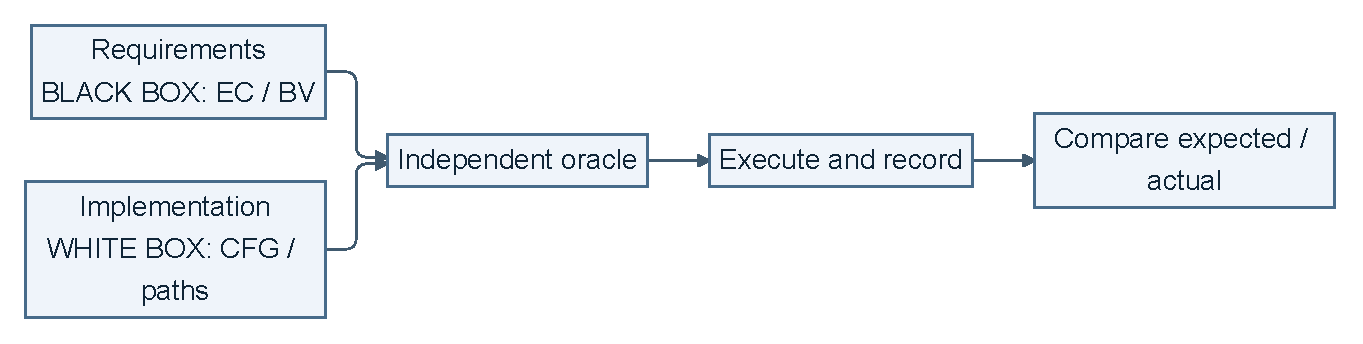
\includegraphics[width=400.66pt]{images/fig-033.pdf}
\captionof{figure}{separate test selection from code coverage}\end{minipage}\par\smallskip

\begin{studycolumns}
\vspace{0pt}



\needspace{4\baselineskip}
\subsection*{12.1 Definitions}
\sectionlabel{h-121-definitions}

\begin{quote}\small\color{navy}
A \textbf{software bug} is \emph{an error, flaw, failure or fault in a computer program or system that causes it to produce an incorrect or unexpected result, or to behave in unintended ways.}

\end{quote}


\begin{quote}\small\color{navy}
\textbf{Software testing} is \emph{an investigation conducted to provide stakeholders with information about the quality of the software product or service under test.}

\end{quote}
Three properties that decide many MCQs:

\begin{enumerate}
\item It is \textbf{dynamic execution} (you run the software).
\item It aims \textbf{to find bugs, not to prove that no bugs exist} (Dijkstra).
\item It reduces the \textbf{perceived risk} of the system not working to an acceptable value.
\end{enumerate}
\textbf{Not testing:} testing \ensuremath{\neq} debugging. Testing finds the failure; debugging locates and fixes the fault.

\needspace{4\baselineskip}
\subsection*{12.2 Why exhaustive testing is impossible}
\sectionlabel{h-122-why-exhaustive-testing-is-impossible}
For a 16-bit integer there are \textbf{2\textsuperscript{1}\textsuperscript{6} = 65 536} inputs. Even that is affordable once, but for realistic signatures the input space is astronomically large, so we must \textbf{select} inputs cleverly. That selection is exactly what \textbf{EC} and \textbf{BV} testing formalise.

\textbf{Selection rule:} random samples can miss the small regions where a defect changes output; use EC/BV to target those regions.
\end{studycolumns}

\Needspace{4\baselineskip}
\subsection*{12.3 Black box vs white box}
\sectionlabel{h-123-black-box-vs-white-box}


{\fontsize{9}{11}\selectfont
\begin{longtable}{L{\dimexpr 0.19829\linewidth-4.76pt\relax}L{\dimexpr 0.46795\linewidth-11.23pt\relax}L{\dimexpr 0.33377\linewidth-8.01pt\relax}}
\toprule
\rowcolor{ice}\textbf{} & \textbf{\textbf{Black box}} & \textbf{\textbf{White box}} \\
\midrule\endfirsthead
\toprule\rowcolor{ice}\textbf{} & \textbf{\textbf{Black box}} & \textbf{\textbf{White box}} \\
\midrule\endhead
\multicolumn{3}{r}{\scriptsize Continued on next page}\\\endfoot
\bottomrule\endlastfoot
What to analyse & \textbf{Requirements and specifications} & \textbf{Implementation details}, internal paths and structure \\
Example requirement & "The income of an applicant must be between \$1500 and \$8000 per month" & --- \\
Techniques & \textbf{Equivalence class testing, boundary value testing}, state-based testing & \textbf{Control flow testing} (CFG, basis paths), data flow testing \\
Pros & Directs the tester to a \textbf{very small subset} of inputs likely to find bugs; applicable at \textbf{all levels} & Gives a \textbf{coverage} notion \\
Cons & \textbf{Cannot infer code coverage from black-box inputs alone}; EC/\allowbreak{}requirement coverage can still be tracked & Needs code; misses "missing requirement" bugs \\
\end{longtable}
}

\begin{studycolumns}
\vspace{0pt}

\needspace{4\baselineskip}
\subsection*{12.4 Levels of testing (4)}
\sectionlabel{h-124-levels-of-testing-4}

\begin{referenceentries}
\textit{\textbf{Level} / \textbf{Scope}}\par\smallskip
\noindent \textbf{\textbf{Unit testing}}: Test a unit individually (the level used in this course)\par
\noindent \textbf{\textbf{Integration testing}}: Test units \textbf{in combination}\par
\noindent \textbf{\textbf{System testing}}: Everything: functionality, usability, reliability, performance, portability, security\ldots{}\par
\noindent \textbf{\textbf{Acceptance testing (UAT)}}: Customer accepts the software and pays\par
\end{referenceentries}
\needspace{4\baselineskip}
\subsection*{12.5 Ingredients of a test case (5 --- memorise)}
\sectionlabel{h-125-ingredients-of-a-test-case-5--memorise}

\begin{referenceentries}
\textit{\textbf{Ingredient} / \textbf{Description}}\par\smallskip
\noindent \textbf{\textbf{Name}}: Distinct name of the test case\par
\noindent \textbf{\textbf{Location}}: Path to the test program and its inputs\par
\noindent \textbf{\textbf{Input}}: Input data or commands\par
\noindent \textbf{\textbf{Oracle}}: \textbf{Expected} test output\par
\noindent \textbf{\textbf{Log}}: \textbf{Actual} output produced by the test\par
\end{referenceentries}
JUnit mapping: \code{@Test public void test\allowbreak{}Qualified\allowbreak{}Application()} = \textbf{Name}; the class/\allowbreak{}package = \textbf{Location}; the arguments to \code{analyze\allowbreak{}Application(.\allowbreak{}.\allowbreak{}.\allowbreak{})} = \textbf{Input}; the expected argument in \code{assert\allowbreak{}Equals(Application\allowbreak{}Result.\allowbreak{}Approval,\allowbreak{} result)} = \textbf{Oracle}; the recorded actual \code{result} and test report = \textbf{Log}.


\begin{quote}\small\color{navy}
\textbf{Trap:} \emph{oracle} = expected; \emph{log} = actual. Keep this distinction when naming test-case components.

\textbf{Oracle check:} derive expected behaviour from requirements; separately validate wrong requirements with stakeholders.

\end{quote}
\end{studycolumns}

\Needspace{4\baselineskip}
\subsection*{12.6 Execution order: cascading vs independent tests}
\sectionlabel{h-126-execution-order-cascading-vs-independent-tests}


{\fontsize{9}{11}\selectfont
\begin{longtable}{L{\dimexpr 0.20210\linewidth-4.85pt\relax}L{\dimexpr 0.41868\linewidth-10.05pt\relax}L{\dimexpr 0.37922\linewidth-9.10pt\relax}}
\toprule
\rowcolor{ice}\textbf{} & \textbf{\textbf{Cascading (dependent)}} & \textbf{\textbf{Independent}} \\
\midrule\endfirsthead
\toprule\rowcolor{ice}\textbf{} & \textbf{\textbf{Cascading (dependent)}} & \textbf{\textbf{Independent}} \\
\midrule\endhead
\multicolumn{3}{r}{\scriptsize Continued on next page}\\\endfoot
\bottomrule\endlastfoot
Shape & Create \ensuremath{\rightarrow} Read \ensuremath{\rightarrow} Update \ensuremath{\rightarrow} Delete \ensuremath{\rightarrow} Read-deleted (each builds on the last) & Self-contained cases for each feature \\
YES Benefit & \textbf{Smaller and simpler} test cases; realistic end-to-end sequence & \textbf{Parallel} test execution; failures are isolated \\
NO Cost & \textbf{One failure invalidates subsequent tests} & \textbf{Larger and more complex} test cases (each sets up its own state) \\
\end{longtable}
}

\begin{studycolumns}
\vspace{0pt}

\needspace{4\baselineskip}
\subsection*{12.7 Basis path testing (white box)}
\sectionlabel{h-127-basis-path-testing-white-box}

\begin{quote}\small\color{navy}
\textbf{Basis path testing} (structured testing) is a white-box method for designing test cases intended to exercise a \textbf{basis set of linearly independent control-flow paths}.

\end{quote}
Process:

\begin{enumerate}
\item Draw the \textbf{Control Flow Graph (CFG)}.
\item Compute the \textbf{Cyclomatic Complexity (CC)}.
\item Derive a set of \textbf{linearly independent paths} (the basis set) --- there are \textbf{CC} of them.
\item Generate a test case for \textbf{each} basis path.
\end{enumerate}
\textbf{Cyclomatic complexity (three equivalent formulas):}


\begin{ReferenceCode}
CC = E - N + 2        (E = edges, N = nodes; per connected component, P components -> +2P)
CC = number of binary decision nodes + 1   (one connected CFG)
CC = number of bounded regions + 1
\end{ReferenceCode}
For a connected, single-entry/\allowbreak{}single-exit CFG, CC is the number of paths in a \textbf{graph basis}. It is \textbf{not} a minimum for statement or branch coverage. Some graph paths are infeasible because of program data, so a structural basis is not automatically an executable test suite. L16, p. 10, loosely says ``all possible paths''; p. 11 illustrates a basis set instead. Loops can create infinitely many execution paths, so these are different coverage goals.

\textbf{Worked CFG:} Section 12.9 distinguishes graph bases from feasible execution and minimum coverage suites.
\end{studycolumns}

\Needspace{4\baselineskip}
\subsection*{12.8 Coverage criteria}
\sectionlabel{h-128-coverage-criteria}


{\fontsize{9}{11}\selectfont
\begin{longtable}{L{\dimexpr 0.26822\linewidth-6.44pt\relax}L{\dimexpr 0.39315\linewidth-9.44pt\relax}L{\dimexpr 0.33864\linewidth-8.13pt\relax}}
\toprule
\rowcolor{ice}\textbf{Criterion} & \textbf{Requirement} & \textbf{Implication} \\
\midrule\endfirsthead
\toprule\rowcolor{ice}\textbf{Criterion} & \textbf{Requirement} & \textbf{Implication} \\
\midrule\endhead
\multicolumn{3}{r}{\scriptsize Continued on next page}\\\endfoot
\bottomrule\endlastfoot
\textbf{Statement coverage} & Every \textbf{node} executed at least once & Weakest; misses branch-only bugs \\
\textbf{Branch (decision) coverage} & Every \textbf{edge} (true and false of every decision) taken at least once & \textbf{100\% branch \ensuremath{\Rightarrow} 100\% statement}, but not vice versa \\
\textbf{Path coverage} & Every \textbf{path} executed & Usually infeasible (loops \ensuremath{\Rightarrow} infinite paths) \\
\textbf{Basis-path coverage} & A feasible independent path set exercised; report infeasible structural paths & Practical middle ground \\
\end{longtable}
}

\begin{studycolumns}
\vspace{0pt}


\begin{quote}\small\color{navy}
\textbf{Trap:} "statement coverage implies branch coverage" is \textbf{false} (a \code{if} with no \code{else} whose body always executes gives 100\% statement but not 100\% branch). The reverse \emph{is} true.

\end{quote}
\needspace{4\baselineskip}
\subsection*{12.9 Worked white-box example you should be able to reproduce --- Tutorial 9}
\sectionlabel{h-129-worked-white-box-example-you-should-be-able-to-reproduce--tutorial-9}

\begin{ReferenceCode}
public int sum(int n, int upperbound){
 1  int result, i;
 2  result = 0;
 3  i = 0;
 4  if(n < 0) {
 5    n = -n;
 6  }
 7  while(i<n && result <= upperbound){
 8    i = i + 1;
 9    result = result + i;
10  }
11  if(result <= upperbound){
12    System.out.println("The sum is " + result);
13  } else {
14    System.out.println("The sum is too large!");
15  }
16  return result;
}
\end{ReferenceCode}
\textbf{CFG} --- 12 nodes (1, 2, 3, 4, 5, 7, 8, 9, 11, 12, 14, 16); the compound \code{while} guard is \textbf{one} node:


\needspace{273pt}
\par\smallskip\noindent\begin{minipage}{\linewidth}\centering
\begin{minipage}[t]{0.488\linewidth}\centering\scriptsize\textbf{1}\par\smallskip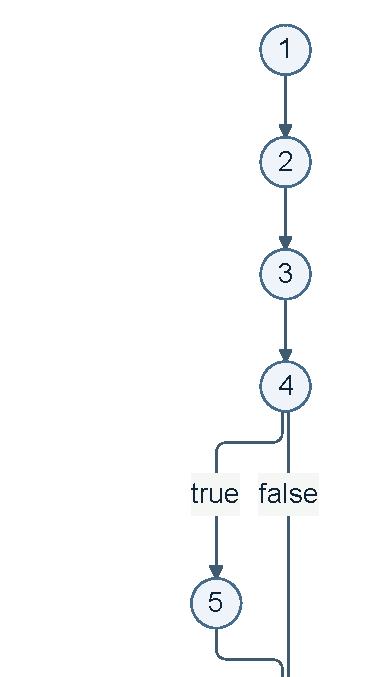
\includegraphics[width=108.10pt]{images/fig-035-compact-1.pdf}\end{minipage}\hfill
\begin{minipage}[t]{0.488\linewidth}\centering\scriptsize\textbf{2}\par\smallskip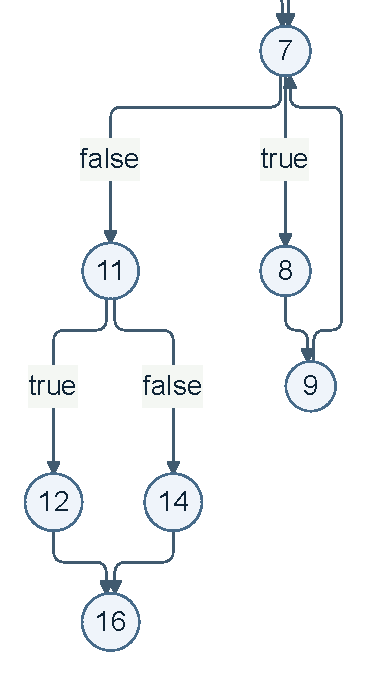
\includegraphics[width=108.10pt]{images/fig-035-compact-2.pdf}\end{minipage}
\captionof{figure}{12.9 Worked white-box example you should be able to reproduce --- Tutorial 9 --- follow numbered panels; crossing arrows continue.}\end{minipage}\par\smallskip


Exact edge list: \code{1\ensuremath{\rightarrow}2,\allowbreak{} 2\ensuremath{\rightarrow}3,\allowbreak{} 3\ensuremath{\rightarrow}4,\allowbreak{} 4\ensuremath{\rightarrow}5,\allowbreak{} 4\ensuremath{\rightarrow}7,\allowbreak{} 5\ensuremath{\rightarrow}7,\allowbreak{} 7\ensuremath{\rightarrow}8,\allowbreak{} 7\ensuremath{\rightarrow}11,\allowbreak{} 8\ensuremath{\rightarrow}9,\allowbreak{} 9\ensuremath{\rightarrow}7,\allowbreak{} 11\ensuremath{\rightarrow}12,\allowbreak{} 11\ensuremath{\rightarrow}14,\allowbreak{} 12\ensuremath{\rightarrow}16,\allowbreak{} 14\ensuremath{\rightarrow}16}.

\textbf{N = 12, E = 14 \ensuremath{\Rightarrow} CC = E \ensuremath{-} N + 2 = 14 \ensuremath{-} 12 + 2 = 4.} \emph{(Cross-check by predicates: \code{if(n<0)}, the \code{while}, \code{if(result <=\allowbreak{} upperbound)} = 3 decisions \ensuremath{\Rightarrow} 3 + 1 = 4.)}

\textbf{One feasible basis set for the combined-guard CFG (CC = 4):}
\end{studycolumns}


{\fontsize{9}{11}\selectfont
\begin{longtable}{L{\dimexpr 0.09590\linewidth-3.07pt\relax}L{\dimexpr 0.28882\linewidth-9.24pt\relax}L{\dimexpr 0.25186\linewidth-8.06pt\relax}L{\dimexpr 0.36342\linewidth-11.63pt\relax}}
\toprule
\rowcolor{ice}\textbf{\#} & \textbf{Path} & \textbf{Covering input} & \textbf{Expected output} \\
\midrule\endfirsthead
\toprule\rowcolor{ice}\textbf{\#} & \textbf{Path} & \textbf{Covering input} & \textbf{Expected output} \\
\midrule\endhead
\multicolumn{4}{r}{\scriptsize Continued on next page}\\\endfoot
\bottomrule\endlastfoot
1 & 1,2,3,4,7,11,12,16 & n = 0, ub = 100 & prints "The sum is 0", returns 0 \\
2 & 1,2,3,4,7,8,9,7,11,12,16 & n = 1, ub = 100 & prints "The sum is 1", returns 1 \\
3 & 1,2,3,4,5,7,8,9,7,11,12,16 & n = \ensuremath{-}1, ub = 100 & prints "The sum is 1", returns 1 \\
4 & 1,2,3,4,7,8,9,7,11,14,16 & n = 1, ub = 0 & prints "The sum is too large!", returns 1 \\
\end{longtable}
}

\textbf{Statement and branch coverage need only two tests}, not four:




{\fontsize{9}{11}\selectfont
\begin{longtable}{L{\dimexpr 0.30144\linewidth-7.23pt\relax}L{\dimexpr 0.35048\linewidth-8.41pt\relax}L{\dimexpr 0.34807\linewidth-8.35pt\relax}}
\toprule
\rowcolor{ice}\textbf{Input} & \textbf{Executed path} & \textbf{Expected print /\allowbreak{} return} \\
\midrule\endfirsthead
\toprule\rowcolor{ice}\textbf{Input} & \textbf{Executed path} & \textbf{Expected print /\allowbreak{} return} \\
\midrule\endhead
\multicolumn{3}{r}{\scriptsize Continued on next page}\\\endfoot
\bottomrule\endlastfoot
\code{n =\allowbreak{} \ensuremath{-}1,\allowbreak{} upperbound =\allowbreak{} 100} & \code{1,\allowbreak{}2,\allowbreak{}3,\allowbreak{}4,\allowbreak{}5,\allowbreak{}7,\allowbreak{}8,\allowbreak{}9,\allowbreak{}7,\allowbreak{}11,\allowbreak{}12,\allowbreak{}16} & \code{The sum is 1} /\allowbreak{} \code{1} \\
\code{n =\allowbreak{} 5,\allowbreak{} upperbound =\allowbreak{} 1} & \code{1,\allowbreak{}2,\allowbreak{}3,\allowbreak{}4,\allowbreak{}7,\allowbreak{}8,\allowbreak{}9,\allowbreak{}7,\allowbreak{}8,\allowbreak{}9,\allowbreak{}7,\allowbreak{}11,\allowbreak{}14,\allowbreak{}16} & \code{The sum is too large!} /\allowbreak{} \code{3} \\
\end{longtable}
}

\begin{studycolumns}
\vspace{0pt}

Together these cover all executable statements and both outcomes of each of the three combined decisions. Two is minimal because the final \code{if} takes only one outcome per call. Four paths are needed for the \textbf{illustrated basis set}, a stronger, different target. The method returns the sum \textbf{after} it has crossed the bound; it does not clamp the return value to \code{upperbound}.

\textbf{Compound-condition convention:} treating the whole \code{while} guard as node 7 gives \textbf{N = 12, E = 14, CC = 4}. Splitting short-circuit \code{\&\&} into nodes 7a (\code{i<n}) and 7b (\code{result<=\allowbreak{}upperbound}) gives \textbf{N = 13, E = 16, CC = 5}. In the split graph, 7a false skips 7b; 7a true reaches 7b; either false exits to 11. State the convention and make the formula match the graph.

The same two coverage tests above also exercise both outcomes of both operands in the split graph: the first ends with \code{i<n} false; the second ends with \code{i<n} true and \code{result<=\allowbreak{}upperbound} false. If a fifth basis path is requested for that graph, add \code{n =\allowbreak{} 1,\allowbreak{} upperbound =\allowbreak{} \ensuremath{-}1}: it skips the body because 7b is false immediately, prints \code{The sum is too large!} and returns \code{0}.

\textbf{Trace carefully:} \code{n =\allowbreak{} 4} with a large bound executes four iterations. A single iteration can be obtained with \code{n =\allowbreak{} 1} and a non-negative bound; \code{n =\allowbreak{} 2} needs a bound that stops the loop after the first addition. A claimed basis path must either match its stated input exactly or be labelled schematic.
\end{studycolumns}
